\section{Lựa chọn điện trở song song để tuyến tính hóa}

\subsection{Tính toán giá trị điện trở song song}

Theo datasheet của NTCLE100E3,

\begin{equation}
	R_{(T)} = R_{ref} \times e^{A + B/T^{1} + C/T^{2} + D/T^{3}}
	\label{Eq: RTH}
\end{equation}

\[
T_{(R)} = \left( A_{1} + B_{1} \ln^{2} \frac{R}{R_{ref}} - C_{1} \ln^2 \frac{R}{R_{ref}} - D_{1} \ln^3 \frac{R}{R_{ref}} \right)^{-1}
\]

Trong đó:

\begin{itemize}[label=-, leftmargin=2cm]
	\item $A$, $B$, $C$, $D$, $A_{1}$, $B_{1}$, $C_{1}$ và $D_{1}$ là các hằng số dựa vào thông số của vật liệu.
	\item $R_{ref}$ là giá trị điện trở tại nhiệt độ tham chiếu (thường chọn ở $T = 25^{o}C$, $ R_{ref} = R_{25}$).
	\item $T$ là nhiệt độ Kelvin (K). $T(^{o}C) = T(K) - 273.15$.
\end{itemize}

Từ phương trình \ref{Eq: RTH}, 

\[ R_{TH} = R_{25} \times e^{A + B/T^{1} + C/T^{2} + D/T^{3}} \]
\[ V_{e} = I \times \dfrac{R_{TH} \times R_{p}}{R_{TH} + R_{p}} \]

Ta có:

$
	\begin{matrix}
		\dfrac{dV_{e}}{dT} & = & \dfrac{I\times R_{p} \left( R_{TH} \left( -\dfrac{B}{T^{2}} - \dfrac{2C}{T_{3}} - \dfrac{3D}{T^{4}} \right) \left( R_{TH} + R_{p} \right) - R_{TH} \left( -\dfrac{B}{T^{2}} - \dfrac{2C}{T_{3}} - \dfrac{3D}{T^{4}} \right)R_{TH} \right)}{\left(R_{TH} + R_{p}\right)^{2}} \\[10pt]
						   & = & \dfrac{I R_{p}^{2} R_{TH} \left( -\dfrac{B}{T^{2}} - \dfrac{2C}{T_{3}} - \dfrac{3D}{T^{4}} \right)}{\left(R_{TH} + R_{p}\right)^{2}} \hfill
	\end{matrix}
$

$
	\dfrac{d^{2}V_{e}}{d^{2}T} = I R_{p}^{2} \left( \dfrac{ R_{TH} (A_{1}^{2} + A_{2})(R_{TH} + R_{p})^{2} -2(R_{TH} + R_{p})R_{TH}^{2}A_{1}^{2} }{(R_{TH} + R_{p})^{4}} \right)
$

Trong đó,

\begin{itemize}[label=-]
	\item $A_{1} = -\dfrac{B}{T^{2}} - \dfrac{2C}{T^{3}} - \dfrac{ 3D }{ T^{4} }$
	\item $A_{2} = \dfrac{ 2B }{ T^{3} } + \dfrac{ 6C }{ T^{4} } + \dfrac{12D}{T^{5}}$
\end{itemize}

$
\Rightarrow \dfrac{d^{2}V_{e}}{d^{2}T} = I R_{p}^{2} \left( \dfrac{R_{TH}( A_{1}^{2} + A_{2} ) (R_{TH} + R_{p}) - 2R_{TH}^{2} A_{1}^{2}}{ \left(R_{TH} + R_{p}\right)^{3} } \right) 
$

Từ Datasheet của NTCLE100E3 với $R_{25} = 10\,\textsf{k}\Omega$:

\begin{figure}[H]
	\centering
	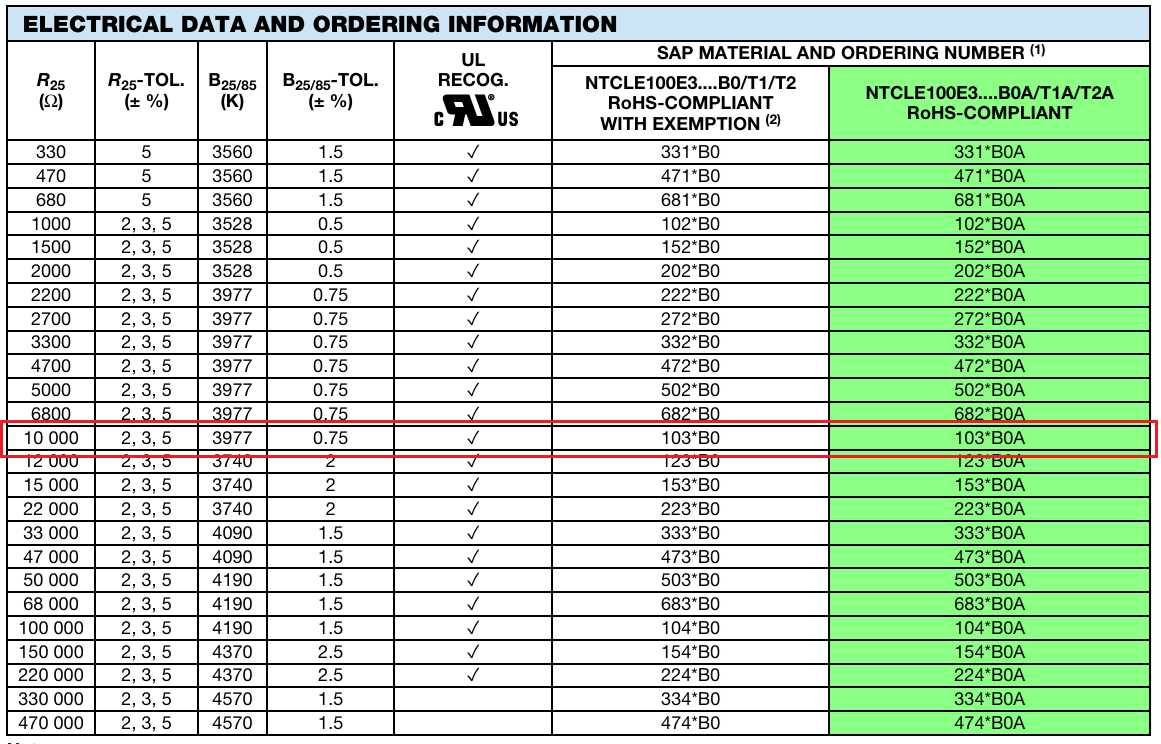
\includegraphics[width=.7\linewidth]{./my-chapters/my-images/Cal_R_parallel/Sel_B_25_85.png}
\end{figure}

Ta chọn được $B_{25/85} = 3977$. Từ đó ta chọn được các giá trị của $A$, $B$, $C$ và $D$ như sau:

\begin{minipage}{.3\linewidth}
	\begin{itemize}[label=-]
		\item $A = -14.6337$
		\item $B = 4791,842$
		\item $C = -115334$
		\item $D = -3730535$
	\end{itemize}
\end{minipage}
\begin{minipage}{.7\linewidth}
	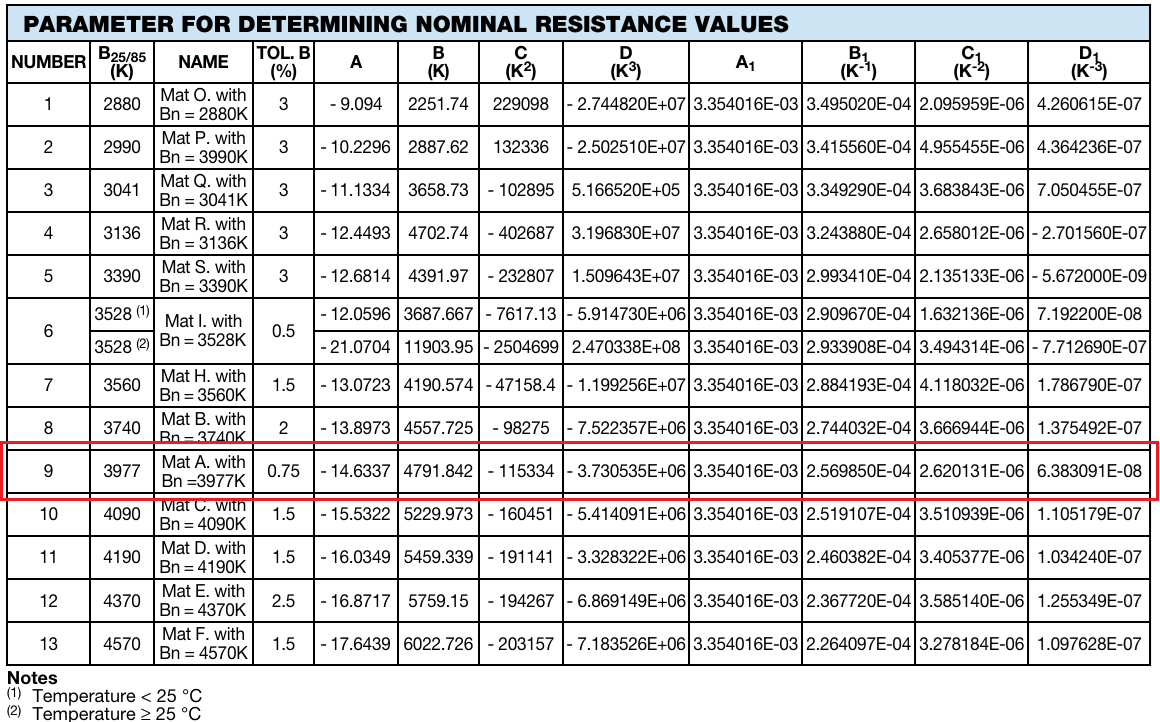
\includegraphics[width=\linewidth]{./my-chapters/my-images/Cal_R_parallel/Sel_ABCD.png}
\end{minipage}

$\Rightarrow 
\left\{ 
	\begin{matrix}
		A_{1} & = & -0.03802560045\\
		A_{2} & = & 2.078383337
	\end{matrix}		
\right. \quad \text{ Tại } T = 50^{o}C = 323.15K
$

Xét $\dfrac{V^{2}V_{e} }{d^{2}T } = 0 \quad \text{ Tại } T = 50^{o}C = 323.15K$.

Từ Datasheets, 

\begin{figure}[H]
	\centering
	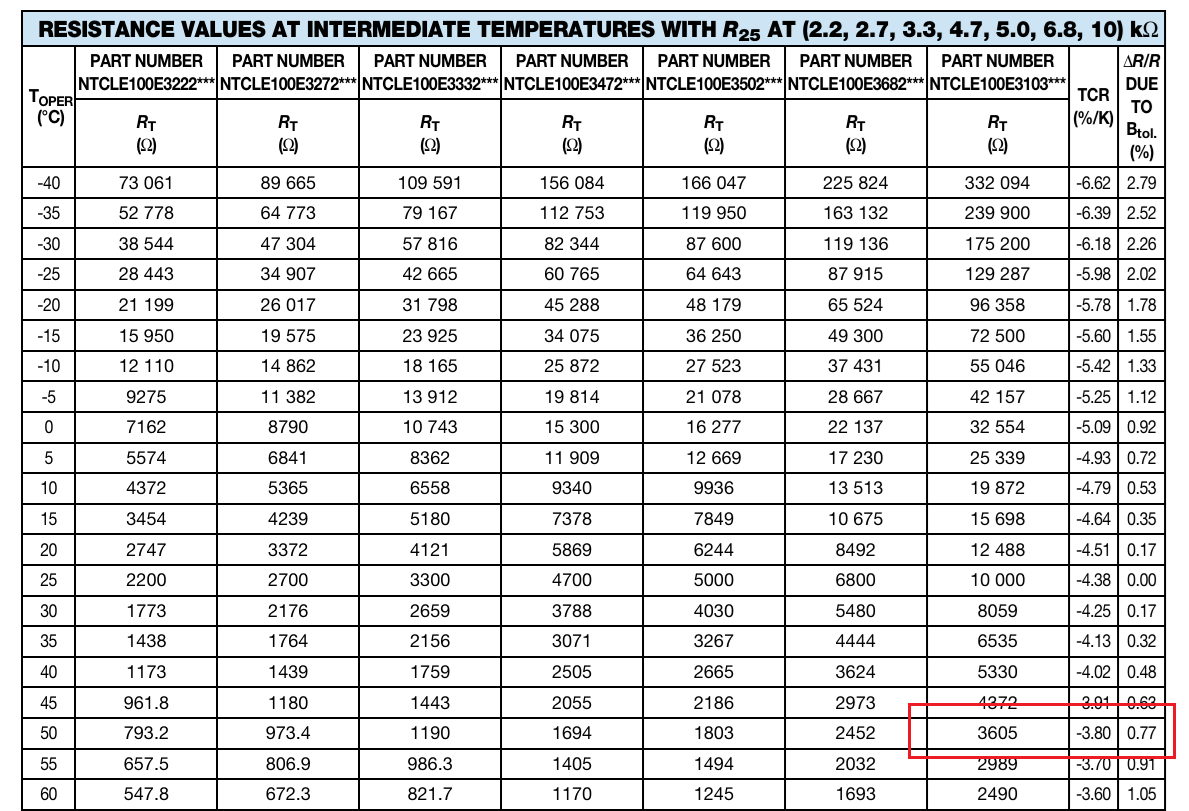
\includegraphics[width=.7\linewidth]{./my-chapters/my-images/Cal_R_parallel/Sel_R_50.png}
\end{figure}

Ta có $R_{50} = 3605\,\Omega$.

$
	\begin{matrix}
		\Rightarrow & R_{p}^{2} R_{TH} \left( A_{1}^{2} + A_{2} \right) \left( R_{TH} + R_{p} \right) - 2 R_{p}^{2} R_{TH}^{2} A_{1}^{2} \hfill & = & 0 \\[6pt]
		\Leftrightarrow & R_{p}^{2} R_{50} \left( A_{1}^{2} + A_{2} \right) \left( R_{50} + R_{p} \right) - 2 R_{p}^{2} R_{50}^{2} A_{1}^{2} \hfill& = & 0 \\[6pt]
		\Leftrightarrow & R_{p}^{3} 5.962 - 16090 R_{p}^{2} \hfill & = & 0
	\end{matrix}
$

$\Rightarrow$ \finalresult{R_{p} = 2.698\,\textsf{k}\Omega \approx 2.7\,\textsf{k}\Omega}

\subsection{Thiết kế mạch cho việc đo Sensor NTCLE100E3 ở lý tưởng}

\begin{figure}[H]
	\centering
	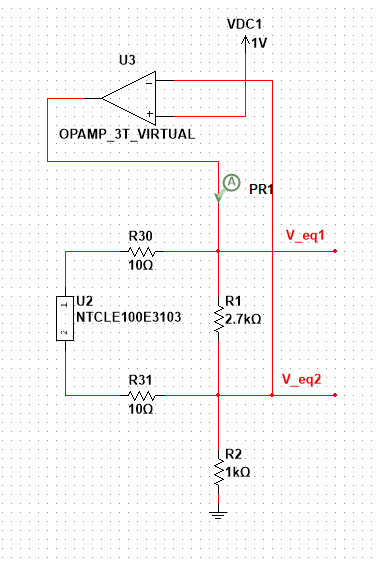
\includegraphics[width=.7\linewidth]{./my-chapters/my-images/Cal_R_parallel/Schematic_current.png}
	\caption{Mạch sau khi tuyến tính hóa bằng điện trở song song.}
\end{figure}

Thực hiện đo điện áp chênh lệch giữa hai đầu điện trở $R_{1}$,
\begin{figure}[H]
	\centering
	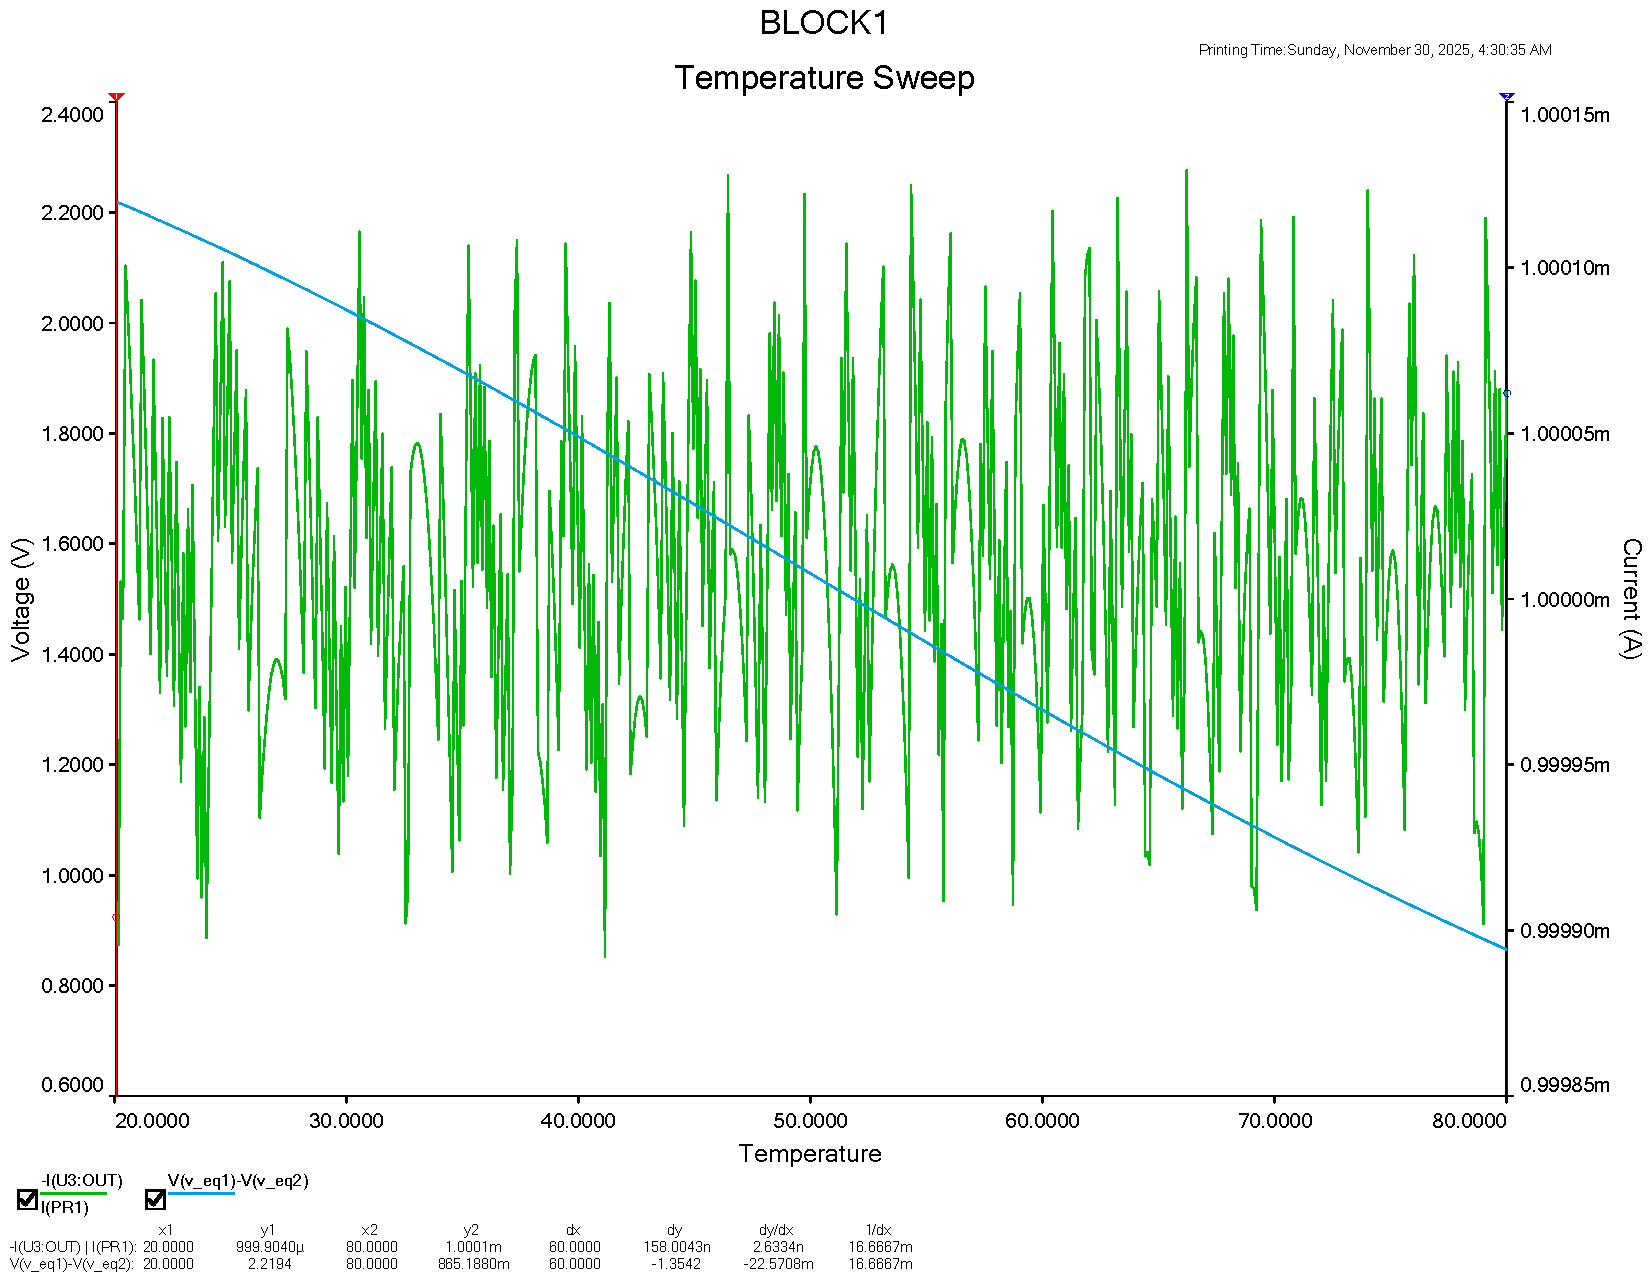
\includegraphics[width=\linewidth]{./my-chapters/my-sim/R_eq_sim.pdf}
	\caption{Điện áp và Dòng điện sau khi tuyến tính hóa.}
\end{figure}

Từ điện áp $V_{eq1} - V_{eq2}$ và $I_{const}$ ta suy ra được giá trị của $R_{eq}$ khi nhiệt độ thay đổi từ $20\rightarrow 80 ^{o}C$: $R_{eq} = \dfrac{V_{eq1} - V_{eq2}}{I_{const}}$, xuất các dự liệu trên vào excel và thuyến tính hóa ta có hình như sau:

\begin{figure}[H]
	\centering
	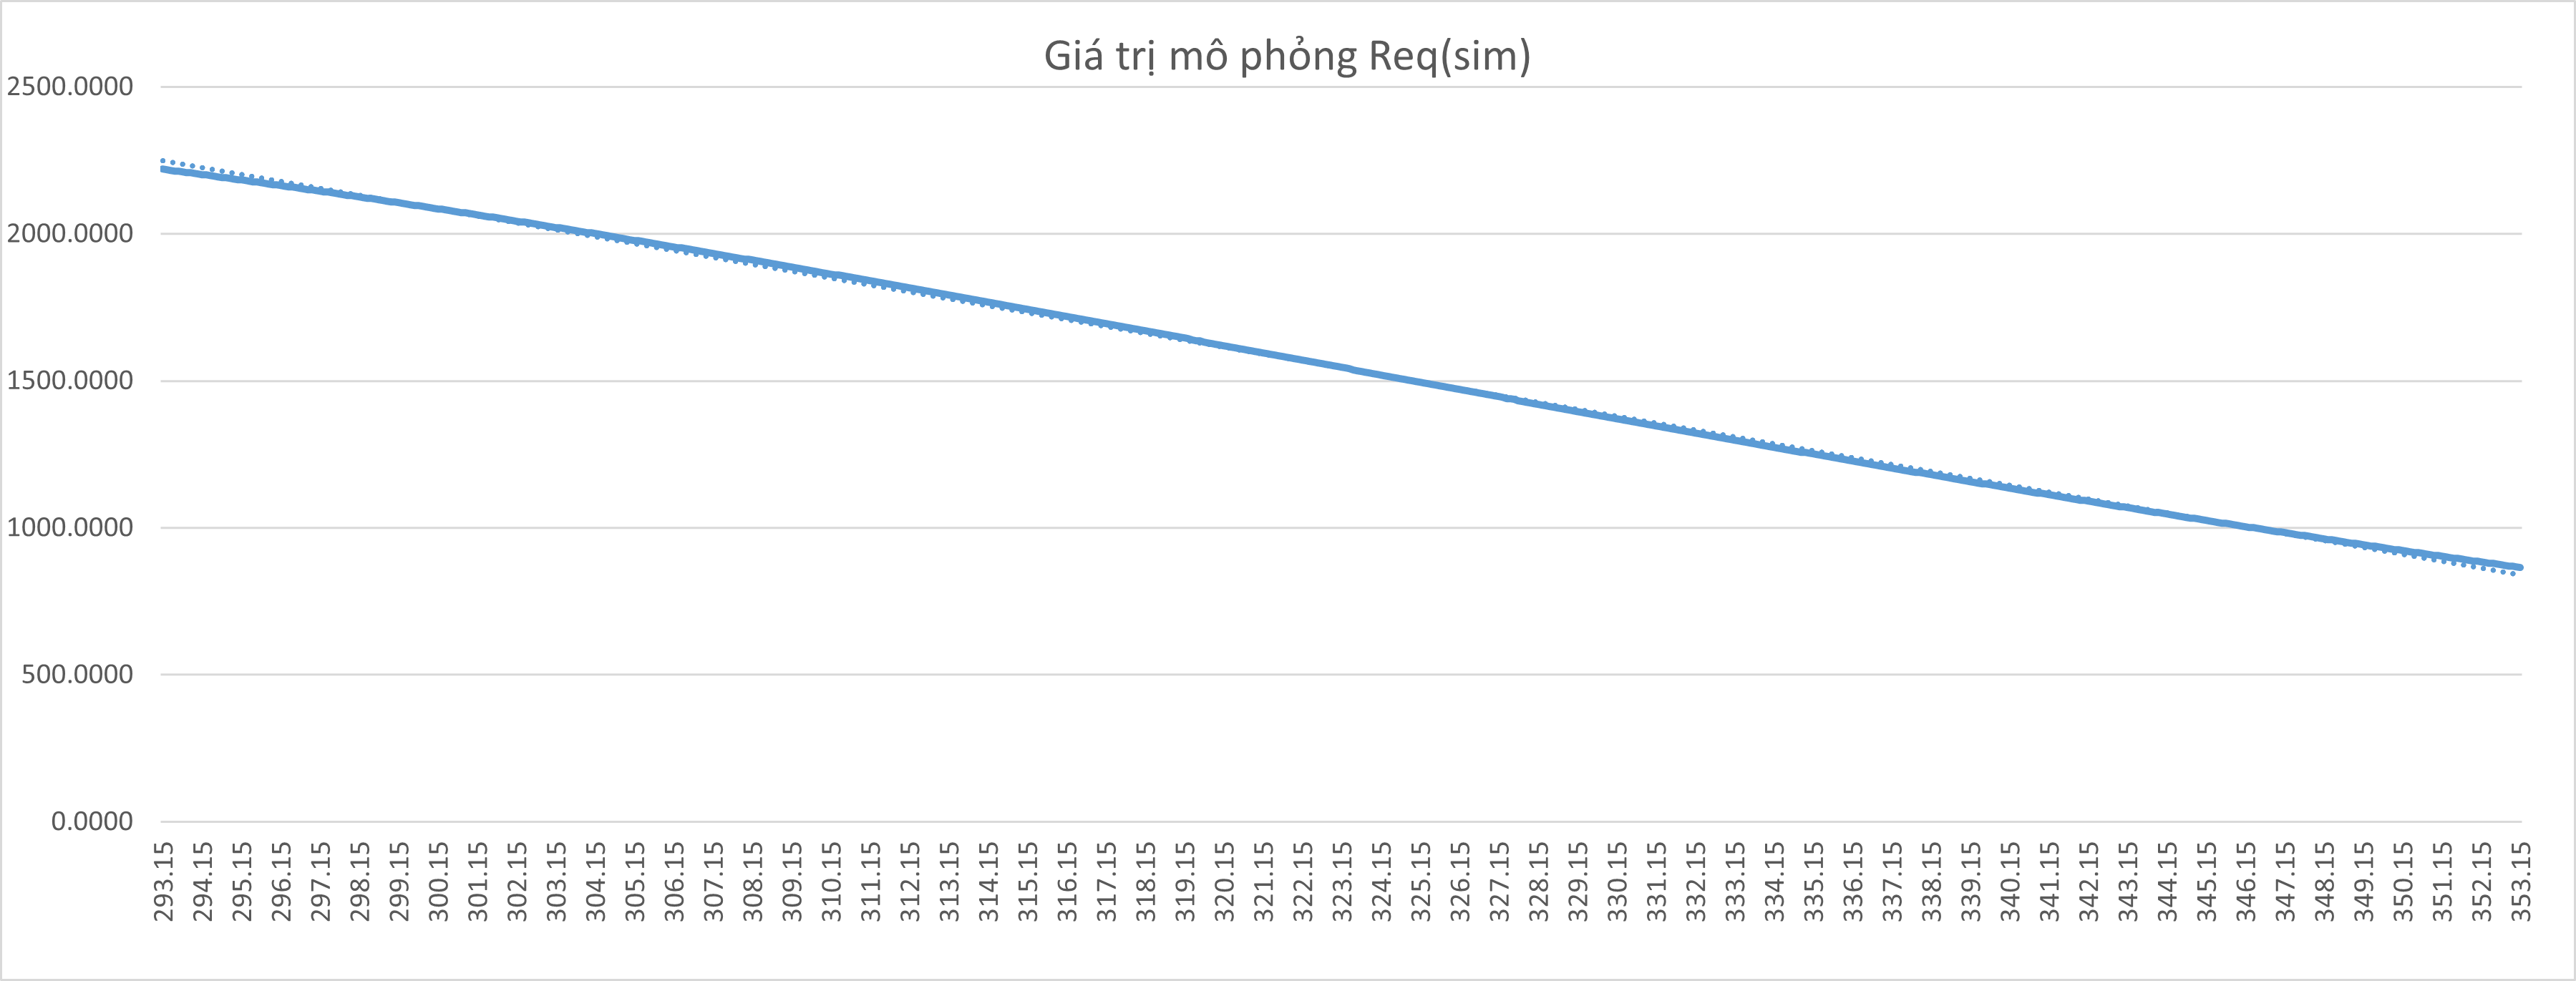
\includegraphics[width=\linewidth]{./my-chapters/my-sim/R_eq_sim.png}
	\caption{Phương trình của $R_{eq}$ và $T (K)$ khi có nhiệt độ thay đổi.}
\end{figure}

Từ đó ta có phương trình tuyến bằng cách sử dụng hàm sau trong excel trên toàn giá trị:

\begin{itemize}[label=-]
	\item \texttt{A = SLOPE(I:I,B:B)} = -23.49111919
	\item \texttt{B = INTERCEPT(I:I,B:B)} = 9136.239792
\end{itemize}

\noindent$\Rightarrow$ Phương trình điện trở $R_{eq}$ theo nhiệt độ như sau: \finalresult{R_{eq} = -23.49111919 \times T(K) + 9136.239792 \,(\Omega) }.

Giả sử với $I_{const} = 1\,\textsf{mA}$ trong khoảng nhiệt độ thì ta có phương trình của $V_{NTC}$ (Với $V_{NTC} = V_{eq1} - V_{eq2}$) là: \finalresult{V_{NTC} = -0.02349 \times T(K) + 9.1362 \,(\textsf{V}) }. 

Theo yêu cầu của đề bài ta có, phương trình liên hệ giữa $T (K)$ ở ngõ vào so với $V_o$ ở ngõ ra bằng phương trình:

\begin{itemize}[label=-]
	\item $\texttt{A} = \dfrac{5 - 0}{353.15 - 293.15} = \dfrac{1}{12} \approx 0.08333$
	\item $\texttt{B} = 0 - A\times 293.15 = -\dfrac{5863}{240} \approx -24.4292$
\end{itemize}

\noindent$\Rightarrow$ \finalresult{V_o = \dfrac{1}{12} \times T - \dfrac{5863}{240}\,(\textsf{V}) \quad \text{ Với } T \text{ là Kelvin}}.

Từ đó, ta có phương trình liên hệ giữa $V_{NTC}$ và $V_{o}$ như sau: \begin{equation}
	\finalresult{V_o = -3.5478\times V_{NTC} + 7.9811 \,(\textsf{V}) }
	\label{Eq: vo relate vntc}
\end{equation}.

\subsection{Thiết kế mạch tổng quát ở lý tưởng}

\begin{figure}[H]
	\centering
	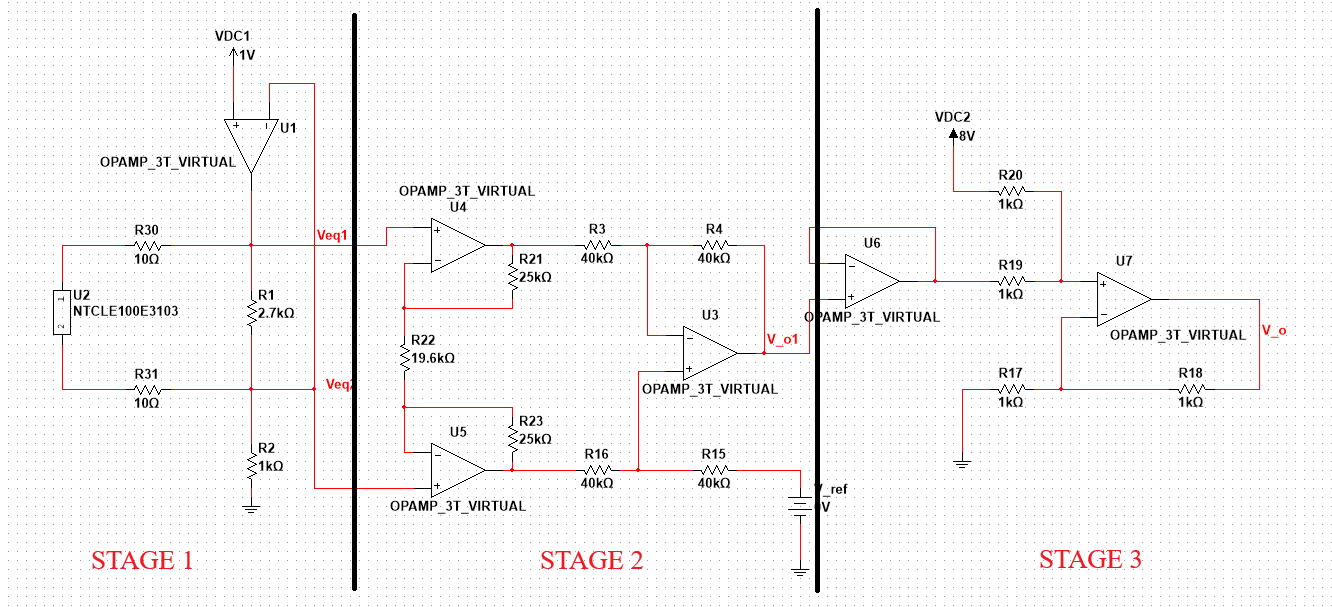
\includegraphics[width=.9\linewidth]{./my-chapters/my-images/Cal_Circuit_Ideal/overview_circuit.png}
	\caption{Mạch chuyển đổi $V_{NTC}$ sang $V_{o}$.}
\end{figure}

\begin{enumerate}[label=Tầng \arabic*.]
	\item Giúp tính hóa giá trị điện trở của Sensor trả về và thực hiện cho một nguồn dòng chạy qua để chuyển đổi từ giá trị điện trở sang giá trị điện áp.
	
	\item Giúp đo vi sai giữa hai đầu điện trở Shunt ($R_{eq}$), loại bỏ nhiễu đồng pha, và khuếch đại giá trị điện áp ngõ ra của NTC đã được tuyến tính và chuyển về điện áp. 
	
	Ta có: $V_{o1} = \left(1 + \dfrac{50}{R_{22}}\right) (V_{in}^{+} - V_{in}^{-}) + V_{ref}$. Với $V_o = -3.5478\times V_{NTC} + 7.9811$, 
	\[ \left(1 + \dfrac{50}{R_{22}}\right) = 3.5478 \Rightarrow R_{22} = 19.8\,\textsf{k}\Omega \]
	\item Sử dụng một mạch cộng không đảo điện áp để cộng thêm và một lượng là $V_{o} = V_{o1} + 7.9811\,\textsf{V} \Rightarrow V_{o} \approx V_{o1} + 8\,\textsf{V}$ để có thể hoàn thiện được phương trình quan hệ giữa $V_{o}$ và $V_{NTC}$.
\end{enumerate}

Ta thực hiện mô phỏng cho ngõ ra $V_{o}$ như sau:

\begin{figure}[H]
	\centering
	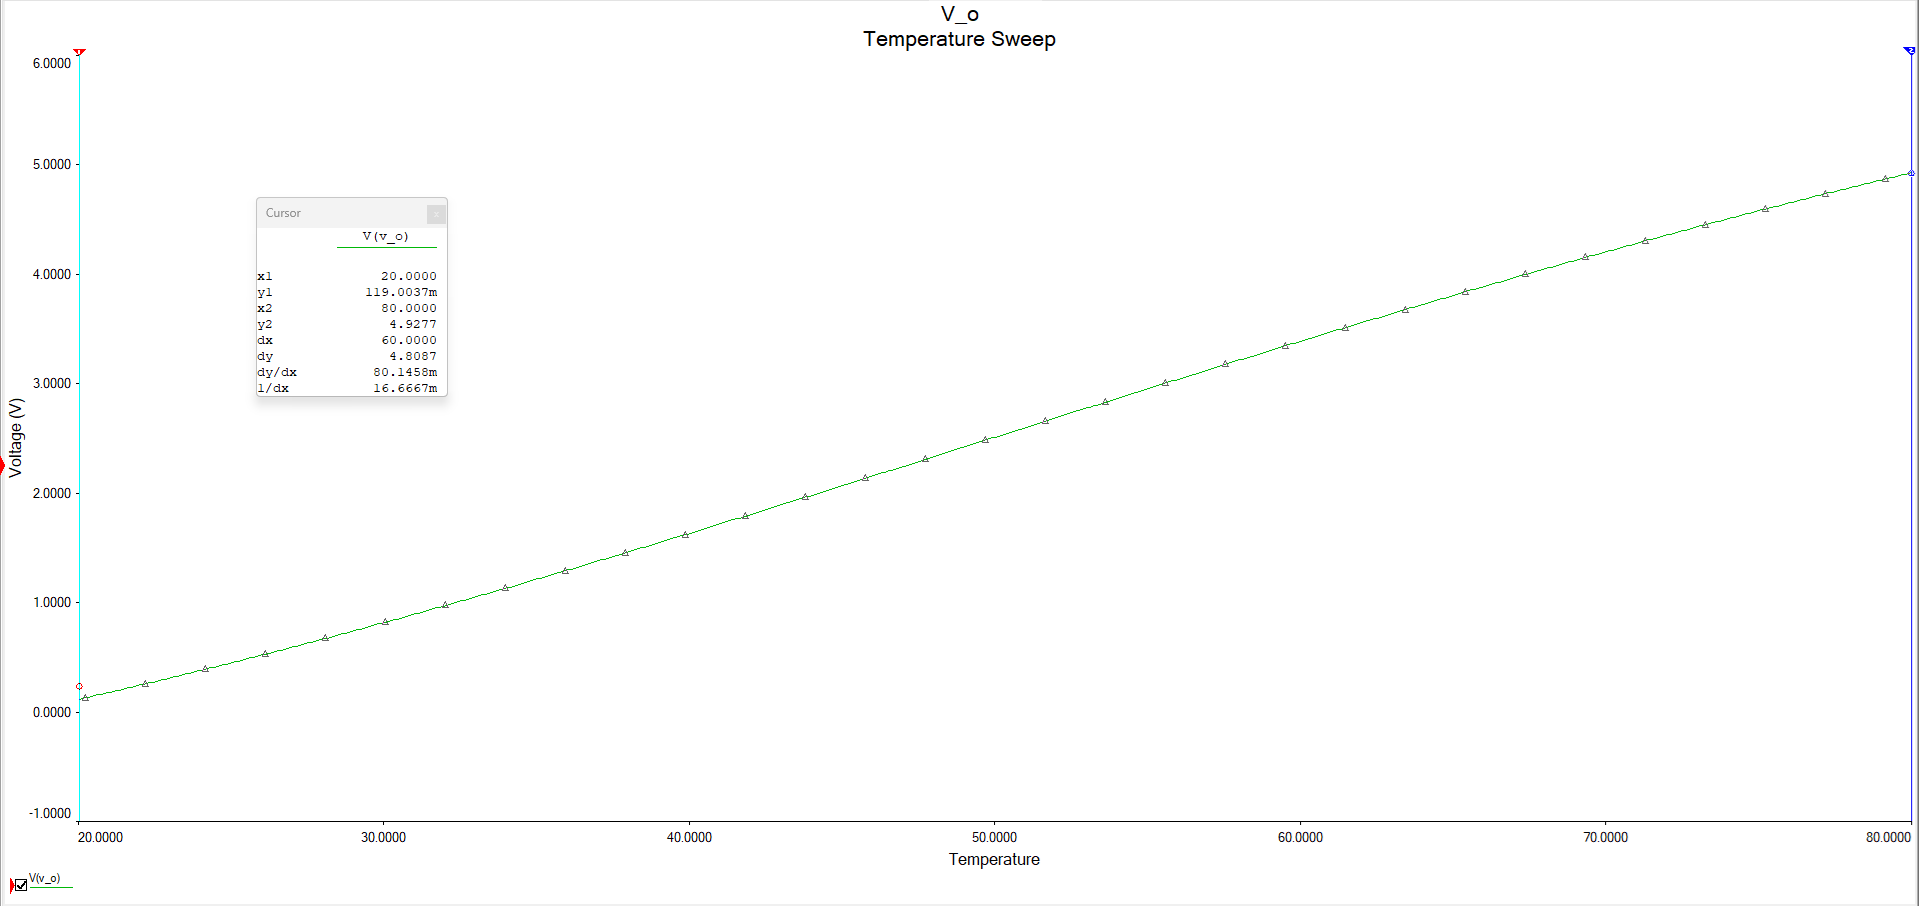
\includegraphics[width=.9\linewidth]{./my-chapters/my-images/Cal_Circuit_Ideal/v_o_before_adjust_value_ina.png}
	\caption{Mô phỏng $V_{o}$ tại trường hợp lý tưởng.}
\end{figure}

Ta thấy:

\begin{itemize}[label=-,leftmargin=2cm]
	\item Tại $20^{o}C (293.15K)$: ta có $V_{o} = 0.119003717218712 \approx 119.0037\,\textsf{mV}$.
	\item Tại $80^{o}C (3353.15K)$: ta có $V_{o} = 4.92774915878843 \approx 4.9277\,\textsf{mV}$.
\end{itemize}

Với sai số lớn, do đề bài yêu cầu sai số là 5\% tức sai số khoảng $1^{o}C \Rightarrow \Delta V_{o} \approx 83.3333\,\textsf{mV}$, nên ta cần điều chỉnh một số thông số để mạch sát với phương trình \ref{Eq: vo relate vntc}:

\begin{figure}[H]
	\centering
	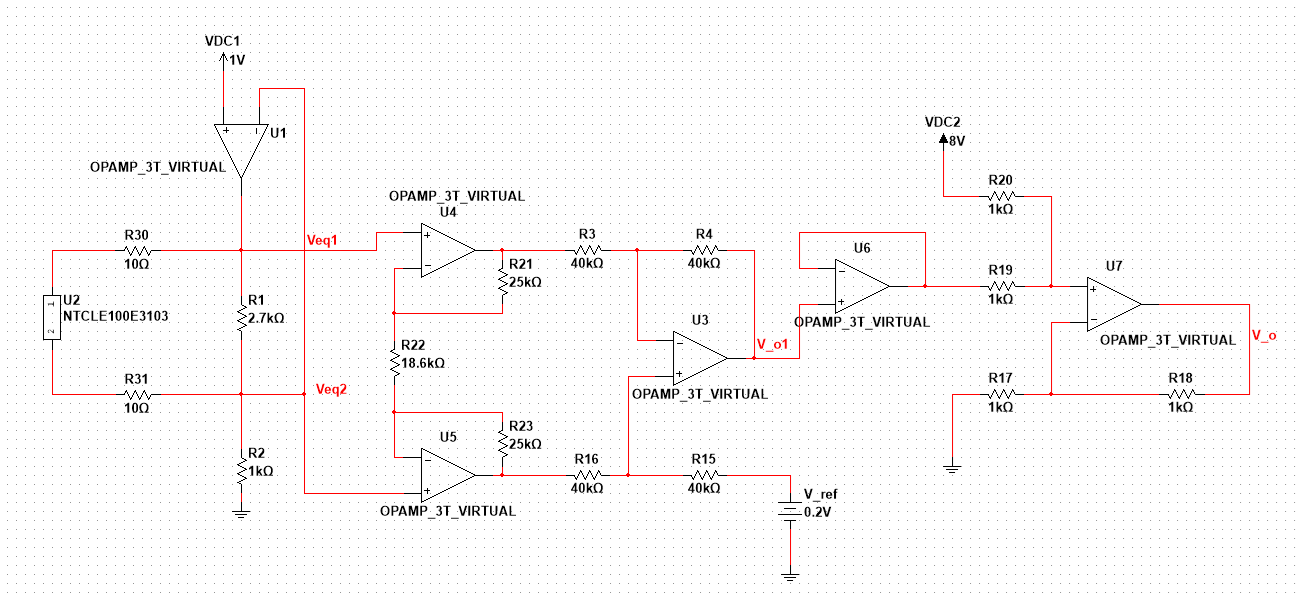
\includegraphics[width=\linewidth]{./my-chapters/my-images/Cal_Circuit_Ideal/circuit_after_adjust.png}
	\caption{Mạch đã điều chỉnh $R_{22}$ và $V_{ref}$ ở tầng khuếch đại vi sai.}
\end{figure}

\begin{figure}[H]
	\centering
	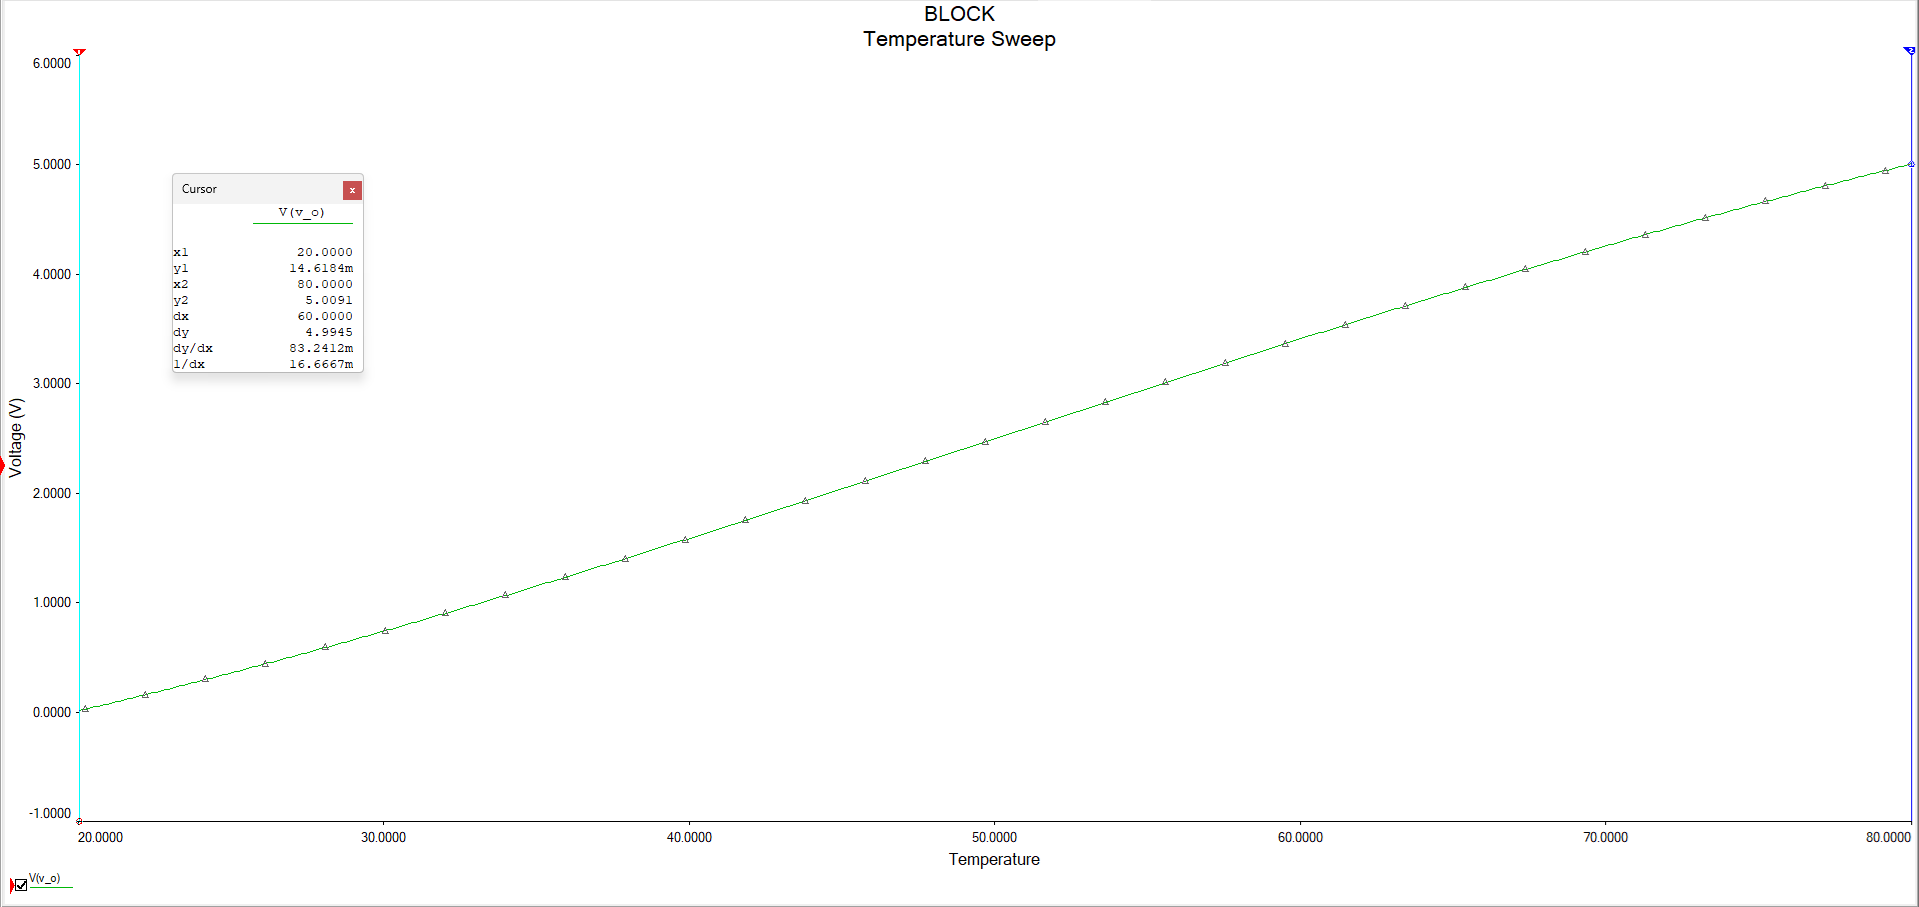
\includegraphics[width=\linewidth]{./my-chapters/my-images/Cal_Circuit_Ideal/v_o_after_adjust_value_ina.png}
	\caption{Mô phỏng $V_{o}$ sau khi điều chỉnh mạch.}
\end{figure}

\begin{itemize}[label=-,leftmargin=2cm]
	\item Tại $20^{o}C (293.15K)$: ta có $V_{o} = 0.014618 \approx 14.618\,\textsf{mV}$.
	\item Tại $80^{o}C (3353.15K)$: ta có $V_{o} = 5.009092 \approx 5.0091\,\textsf{mV}$.
\end{itemize}
%\newpage
%\begin{landscape}
%	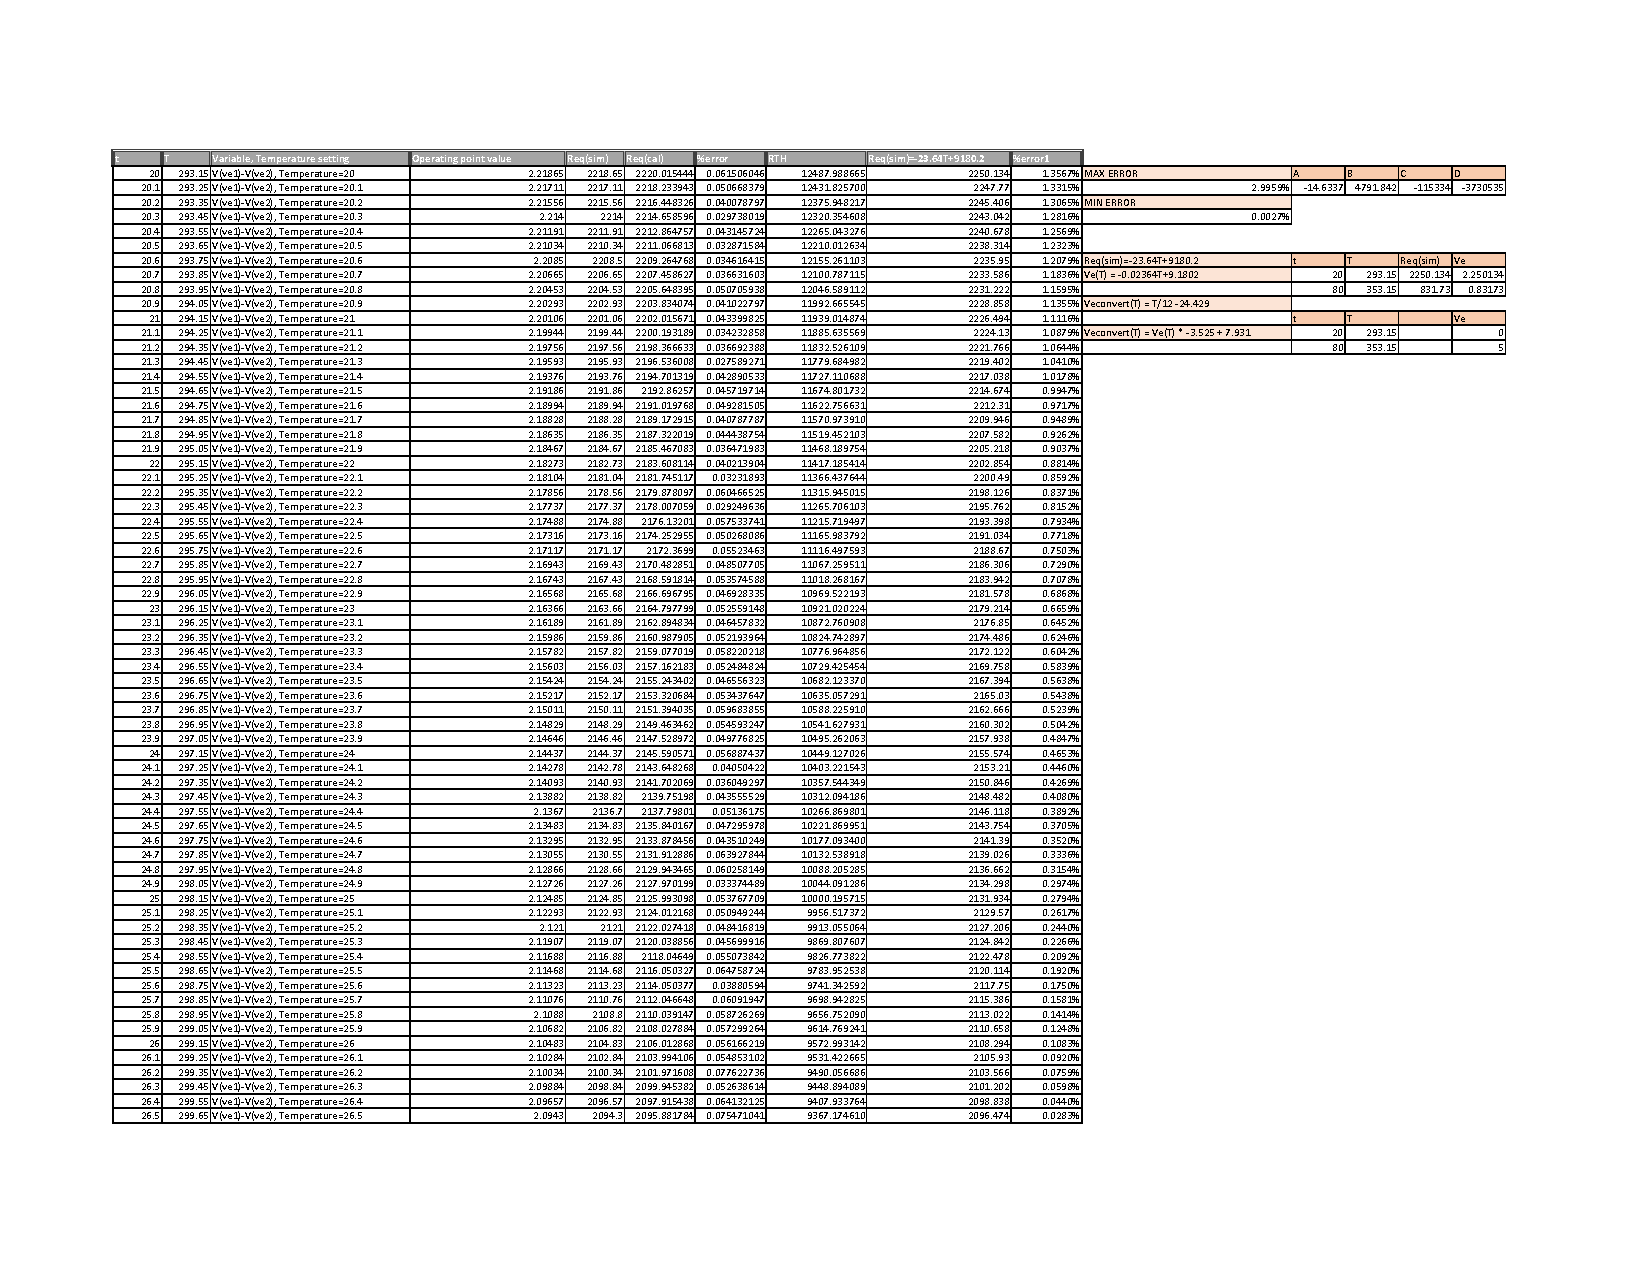
\includepdf[pages=-,angle=90,offset=0cm 0cm]{./my-chapters/my-images/Cal_R_parallel/Export_Cal_R_parallel.pdf}
%\end{landscape}
%\newpage